% SARA -- journal article (Elsevier elsarticle, preprint, numbered references).
% Every number is taken from the thesis results chapter; see ../../02_RESULTS_MASTER_TABLE.md for the source of each.
% Compile: pdflatex main ; bibtex main ; pdflatex main ; pdflatex main
%
% Highlights (Elsevier asks for a separate file; at most 85 characters each):
%  - An offline Bangla assistive smart glass runs five modes on a Raspberry Pi 5
%  - Multi-view counterfeit models collapse with fewer views; prefix training fixes it
%  - A serial audit shows the standard JaalTaka split tests known counterfeit prints
%  - A 47,818-parameter physics-based watermark checker matches a 46x larger CNN
%  - A never-accusing verdict passed 0 of 88 test counterfeits as genuine
\documentclass[preprint,12pt]{elsarticle}
\usepackage{amsmath,amssymb}
\usepackage{graphicx}
\usepackage{booktabs}
\usepackage{multirow}
\usepackage{xcolor}
\usepackage{tikz}
\usetikzlibrary{positioning,arrows.meta}
\usepackage[hidelinks]{hyperref}
\usepackage{lineno}
\usepackage{adjustbox}
\graphicspath{{figures/}}
\emergencystretch=2.5em
\def\UrlBreaks{\do\/\do-\do\_}
\journal{(target journal)}  % TODO: e.g. Engineering Applications of Artificial Intelligence

\begin{document}

\begin{frontmatter}

\title{Seeing Money, Text and Surroundings Offline: A Bangla Assistive Smart Glass with Prefix-Robust Multi-View Counterfeit Screening, Physics-Based Watermark Residuals and a Never-Accusing Verdict}

% TODO: e-mail addresses, ORCIDs, corresponding author.
\author{MD Abdun Fattah Lam}
\author{Mukut Protim Memo}
\author{Tanjila Hossain Tapti}
\author{Mohammad Shidujaman}
\affiliation{organization={Department of Computer Science and Engineering, Independent University, Bangladesh},
            city={Dhaka},
            country={Bangladesh}}

\begin{abstract}
Blind and low-vision people in Bangladesh usually need another person to tell them which banknote they hold, whether it is genuine, what a label says and what is ahead, and the answer cannot be checked. We present SARA (Smart Assistive Reading Aid), a wearable glass that runs entirely on a Raspberry~Pi~5. It speaks Bangla, reads Bangla and English text, names objects, announces facial expressions and recognises Bangladeshi Taka notes; only an optional scene description uses the internet.

Building the currency path produced four findings.
(i) A YOLOv8s detector trained only on 22,333 automatically labelled composites reaches 0.995 mAP@0.5 on held-out composites and names 91.5\% of 1,536 independent photographs correctly. Synthetic hand-held close-ups raise its accuracy on real hand-held notes from 11.8\% to 47.5\%.
(ii) Multi-view counterfeit networks trained with all six views of a note collapse when a user captures fewer, to 71.2\% with one view and with large seed-to-seed swings. A controlled comparison shows that sampling random view prefixes during training alone removes the collapse (98.2\% with one view, three seeds).
(iii) An audit of serial numbers shows that the standard split of the JaalTaka benchmark tests known counterfeit reprints: 279 of 322 readable 500~Taka counterfeits carry one serial, and a serial lookup alone scores 90.2\%. On a print-disjoint split accuracy falls by about eight points, and a watermark check restores it to 95.0\%, level with a properly fine-tuned ResNet-50. A physics-based denomination-matched watermark residual (DMWR) with 47,818 parameters is statistically level with a fine-tuned MobileNetV2 that is 46 times larger.
(iv) A verdict that never says ``counterfeit'' and confirms a note only above the highest validation counterfeit score has a distribution-free pass bound of $1/(n{+}1)$; it passed none of 88 test counterfeits.

For text, region selection reduces the character error rate on a correctly shaped Bangla benchmark from 9.3\% to 2.4\%, and a blended real-word recogniser lowers Bangla error on real street words from 39.2\% to 28.7\%. A currency answer takes 327\,ms on the Pi. We report the limitations equally plainly: no evaluation yet through the glass camera, no completed user study, few counterfeit prints and synthetic voices.
\end{abstract}

\begin{keyword}
assistive technology \sep smart glasses \sep visual impairment \sep banknote recognition \sep counterfeit detection \sep multi-view learning \sep selective prediction \sep Bangla OCR \sep edge AI
\end{keyword}

\end{frontmatter}

\linenumbers

%% ---------------------------------------------------------------------------
\section{Introduction}
\label{sec:intro}

At least 2.2 billion people have a near or distance vision impairment, and its prevalence in low- and middle-income regions is about four times that in high-income regions \cite{who2023vision}. In Bangladesh, three everyday questions usually require help from another person. The first is money: which note was handed back, and is it genuine? The second is reading: what does a medicine label, sign or letter say? The third is the surroundings: what or who is ahead? In each case the blind person depends on an answer they cannot verify.

Existing aids do not close this gap. OrCam MyEye \cite{orcam}, the best-known commercial reading glass, works offline, but Bangla is not among the languages it lists and it does not recognise Taka notes. Research systems based on Google Glass \cite{googleglass2021} or custom wearables such as AIris \cite{airis2024} send pictures to a server. Low-cost Raspberry~Pi reading aids \cite{readingaid_rpi2023,wearable_review2024} are mostly English-only. Work on Bangladeshi counterfeit notes \cite{uddin2016counterfeit,pathak2024counterfeit,chowdhury2022uvink} and the JaalTaka benchmark \cite{jaaltaka,piyas2026jaaltaka} has not been brought to a wearable, and it has not asked how a model behaves when a blind user cannot take every photograph the training data assumes.

This article describes SARA, an offline assistive glass built for this setting, and the four questions its currency path raised. (1) Can a Taka detector be trained without hand labels and still work on real, hand-held photographs? (2) Why do multi-view counterfeit models fail with fewer views, and can training fix it? (3) Does the standard counterfeit benchmark measure what it appears to? (4) How can a device give counterfeit advice that never wrongly accuses a genuine note? We also report the text-reading, object, emotion, voice and on-device results of the complete system.

\textbf{Contributions.}
\begin{enumerate}
\item \emph{System.} A five-mode Bangla assistive glass on a Raspberry~Pi~5 (Section~\ref{sec:system}), with accuracy reported per module and latency, memory and temperature measured on the device (Section~\ref{sec:res_pi}).
\item \emph{Zero-annotation Taka detection.} Copy-paste compositing with exact labels from the paste geometry, and synthetic hand-held close-ups that raise accuracy on independent hand-held photographs about four-fold (Sections~\ref{sec:m_comp}, \ref{sec:res_det}).
\item \emph{View-count collapse.} Jointly trained multi-view fusion networks fail and become seed-unstable when fewer views are available. Prefix sampling alone removes this, as a controlled comparison shows, and the effect does not transfer to every fusion head (Sections~\ref{sec:m_prefix}, \ref{sec:res_views}).
\item \emph{A benchmark shortcut and a stricter split.} A serial-number audit of JaalTaka and a print-disjoint split; watermark checking, including the physics-based DMWR, recovers most of the loss on unseen prints (Sections~\ref{sec:m_serial}--\ref{sec:m_dmwr}, \ref{sec:res_unseen}).
\item \emph{A never-accusing verdict.} A selective policy with a conformal pass bound, evaluated on close-up and whole-note photographs, together with the negative result that motivated it (Sections~\ref{sec:m_safe}, \ref{sec:res_safe}).
\item \emph{Honest evaluation.} Validation-only selection, single reads of every test set, three seeds, and an audit of every claim against its result file. The corrections this audit forced are reported (Section~\ref{sec:discussion}).
\end{enumerate}

%% ---------------------------------------------------------------------------
\section{Related work}
\label{sec:related}

\textbf{Assistive wearables.} Smart glasses for blind users range from commercial devices (OrCam MyEye \cite{orcam}, Envision \cite{envision}, Seeing AI on a phone \cite{seeingai}) to research prototypes based on Google Glass \cite{googleglass2021}, custom cameras \cite{airis2024,smartglass_mdpi2021} or Raspberry~Pi boards \cite{readingaid_rpi2023,thirdeye2019}. Surveys of the field are given in \cite{wearable_review2024,at_review2025}. Of the systems we reviewed, most rely on English, on a phone or on the cloud, and few report both per-feature accuracy and latency on the worn device. Bangla reading has been addressed with OCR systems \cite{banglaocr2021} but rarely in a wearable.

\textbf{Taka recognition and counterfeit detection.} NSTU-BDTAKA \cite{nstubdtaka2024} provides detection and recognition data and a YOLOv5 baseline trained on 3,111 annotated images. Uddin et~al.\ classified watermark, micro-printing and hologram features of Taka notes with an SVM \cite{uddin2016counterfeit}. Pathak et~al.\ trained CNNs on genuine and counterfeit photographs \cite{pathak2024counterfeit}. Chowdhury et~al.\ used the colour flecks visible only under UV light, reaching 96.3\% with a region proposal network \cite{chowdhury2022uvink}. JaalTaka \cite{jaaltaka,piyas2026jaaltaka} contributes six ordered close-up views of 1,390 genuine notes from government banks and counterfeits seized by the Rapid Action Battalion. Banknote inspection under UV-A light relies on fluorescent fibres in otherwise non-fluorescent paper \cite{mutanen2003luminescent,ecb2010quickguide}.

\textbf{Synthetic data.} Copy-paste augmentation \cite{copypaste2021,cutpaste2017} and domain randomisation \cite{tobin2017domain} train detectors from composites. We use them to remove manual annotation entirely and to simulate hand-held capture.

\textbf{Multi-view learning.} Multi-view CNNs pool per-view features \cite{mvcnn}; modality dropout \cite{moddrop} trains fusion models to tolerate missing inputs. MVP-N \cite{mvpn} and ModelNet \cite{modelnet} are standard multi-view benchmarks. We isolate a specific failure, the collapse of fixed-view training at small view counts, and test which part of the training causes it.

\textbf{Shortcuts and leakage.} Models exploit shortcuts that benchmarks fail to exclude \cite{geirhos2020shortcut}, and leakage between training and test data inflates results across machine-learning-based science \cite{kapoor2023leakage}. Our serial audit is an instance of this problem in currency authentication.

\textbf{Selective prediction.} Classifiers with a reject option date back to Chow \cite{chow1970}; selective networks \cite{selective2017} and conformal prediction \cite{vovk2005} give coverage and error guarantees. We use the simplest such guarantee to bound how often a counterfeit is passed.

%% ---------------------------------------------------------------------------
\section{The SARA system}
\label{sec:system}

\subsection{Hardware}
Table~\ref{tab:hw} lists the components of the second prototype (Fig.~\ref{fig:proto}). The first prototype carried the board and fan on one temple; the second moves the Raspberry~Pi~5 \cite{raspberrypi5} into a ventilated enclosure at the back of the head, which balances the frame and keeps the board's heat away from the face.

\begin{table}[!htbp]
\caption{Hardware of the second prototype}
\label{tab:hw}
\centering\small
\begin{adjustbox}{max width=\textwidth}\begin{tabular}{@{}p{3.4cm}p{6.2cm}p{4.2cm}@{}}
\toprule
Part & Details & Role \\ \midrule
Raspberry Pi 5, active cooler & 4-core 2.4\,GHz, 8\,GB; no accelerator used & Runs all models \\
USB webcam & Logitech C270 (second prototype; Camera Module 2 in the first), used at 640$\times$480 & Text, notes, scenes \\
Five push-buttons & GPIO 17, 27, 24, 22, 23: MODE, ACTION, READ, VOL+, VOL$-$ & Screen-free control \\
Vibration motor & GPIO 13 & Signals a found note \\
Bone-conduction headphone & Open-ear & Speech, ears stay free \\
UV-A lamp & 360--395\,nm, beside the camera & Optional UV fibre check \\
Frame and rear enclosure & 3D-printed; head strap; ventilated case & Fit, balance, cooling \\
Power bank & USB-C (Pi~5 supply rated 5\,V, 5\,A) & Portable power \\ \bottomrule
\end{tabular}\end{adjustbox}
\end{table}

\begin{figure}[!htbp]
\centering
\includegraphics[width=0.48\textwidth]{sara_v2_collage.jpg}
\caption{Second SARA prototype worn by a team member: camera and UV lamp at the front, five buttons and a bone-conduction headphone along the temple, and the Raspberry~Pi~5 in a rear enclosure.}
\label{fig:proto}
\end{figure}

\subsection{Software and modes}
Fig.~\ref{fig:arch} shows the pipeline. A mode manager on the Pi runs one mode at a time on the CPU, using PyTorch \cite{pytorch} or ONNX Runtime \cite{onnxruntime}, with 8-bit quantisation \cite{jacob2018quantization} where it keeps accuracy. The five modes are as follows.
\begin{itemize}
\item \emph{Text}: CRAFT detection \cite{craft} in ONNX and EasyOCR recognition \cite{easyocr}, with the pipeline of Section~\ref{sec:m_ocr}.
\item \emph{Objects}: YOLOv8s \cite{ultralytics} trained on COCO \cite{coco}, scanning every 1.5\,s and announcing at most three objects above confidence 0.50.
\item \emph{Taka}: the detector of Section~\ref{sec:m_comp}, the count and total of several notes, the safe verdict of Section~\ref{sec:m_safe}, a guided watermark check and an optional UV fibre check.
\item \emph{Emotion}: YuNet face detection \cite{yunet} and an EfficientNet-V2-S \cite{efficientnetv2} trained on RAF-DB \cite{rafdb}.
\item \emph{Online description}: a cloud vision model, the only mode that needs the internet.
\end{itemize}

\begin{figure}[!htbp]
\centering
\resizebox{0.95\textwidth}{!}{%
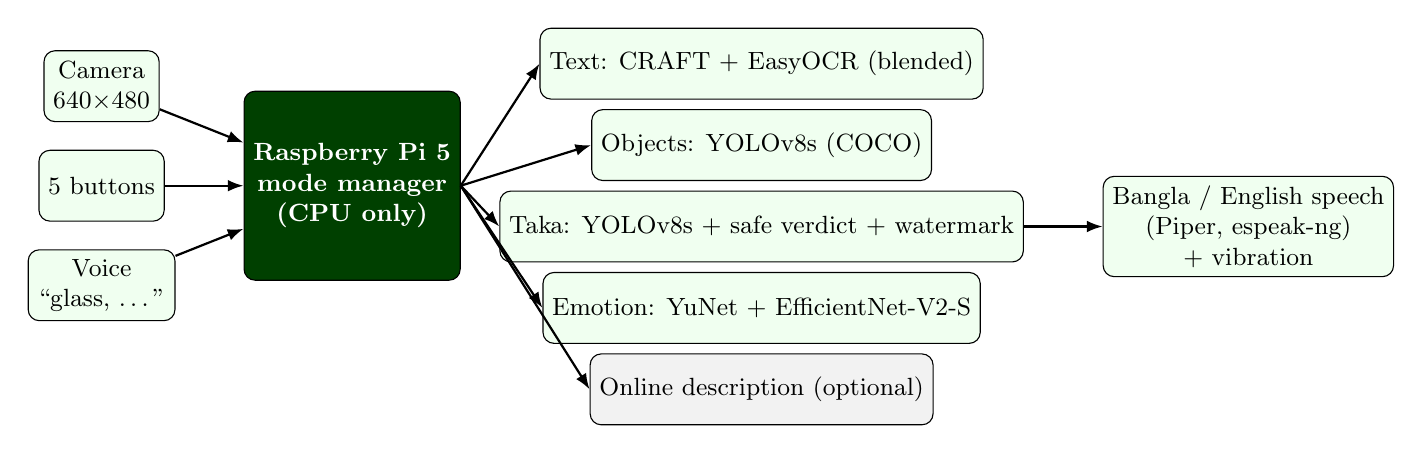
\begin{tikzpicture}[font=\small, node distance=0.35cm and 0.6cm,
  box/.style={draw, rounded corners, align=center, minimum height=0.9cm, fill=green!6},
  pi/.style={draw, rounded corners, align=center, minimum height=2.4cm, fill=green!25!black, text=white, font=\small\bfseries},
  arr/.style={-{Latex[length=2mm]}, thick}]
\node[box] (cam) {Camera\\640$\times$480};
\node[box, below=of cam] (btn) {5 buttons};
\node[box, below=of btn] (mic) {Voice\\``glass, \dots''};
\node[pi, right=1.0cm of btn] (pi) {Raspberry Pi 5\\mode manager\\(CPU only)};
\node[box, right=1.0cm of pi, yshift=1.55cm] (t) {Text: CRAFT + EasyOCR (blended)};
\node[box, below=0.12cm of t] (o) {Objects: YOLOv8s (COCO)};
\node[box, below=0.12cm of o] (c) {Taka: YOLOv8s + safe verdict + watermark};
\node[box, below=0.12cm of c] (e) {Emotion: YuNet + EfficientNet-V2-S};
\node[box, below=0.12cm of e, fill=gray!10] (n) {Online description (optional)};
\node[box, right=1.0cm of c] (sp) {Bangla / English speech\\(Piper, espeak-ng)\\+ vibration};
\foreach \s in {cam,btn,mic} \draw[arr] (\s) -- (pi);
\foreach \m in {t,o,c,e,n} \draw[arr] (pi.east) -- (\m.west);
\draw[arr] (c.east) -- (sp);
\end{tikzpicture}}
\caption{SARA pipeline. All modes except the online description run on the Pi's CPU.}
\label{fig:arch}
\end{figure}

\subsection{Interaction for users without sight}
Each mode is started with a button or a voice command that begins with the wake word ``glass'' (``glass, check money'', ``glass, read text''). Commands are recognised with a closed grammar in Vosk \cite{vosk}: unknown words at the edges of an utterance are dropped, results below a confidence of 0.5 are ignored, and the microphone is muted while the glass speaks. Speech is produced with Piper \cite{piper} in Bangla and English, with espeak-ng \cite{espeakng} as a fall-back. Each sentence is rendered completely and then played at its voice's own sample rate after 150\,ms of silence. This fixed a broken voice on the Pi, where synthesis and playback had run at the same time and one voice had played 38\% too fast. During long captures the glass says ``reading'' and plays a soft tick. A thermal governor reads the temperature every second. It slows the automatic object scan from 1.5\,s to 3\,s above 72\,$^\circ$C and to 6\,s above 77\,$^\circ$C, and pauses it above 81\,$^\circ$C; a button press is never delayed.

%% ---------------------------------------------------------------------------
\section{Data}
\label{sec:data}
Table~\ref{tab:data} lists the datasets. Every split is disjoint by the physical unit (note, writer or print), not by image. An image-level split of JaalTaka gave an accuracy of 1.00 because views of one note appeared in both training and test data; we do not report it. A third public Taka collection was excluded because its files are byte-identical to the training source.

\begin{table}[!htbp]
\caption{Datasets used in this work}
\label{tab:data}
\centering\footnotesize
\begin{adjustbox}{max width=\textwidth}\begin{tabular}{@{}p{3.3cm}p{5.4cm}p{4.9cm}@{}}
\toprule
Dataset & Content & Use and split \\ \midrule
BanglaTaka \cite{banglataka} & 5,073 background-free photos, 9 notes & Composite foregrounds; 80/10/10 by note \\
COCO \cite{coco} & Everyday photos; val2017 (5,000) & Backgrounds; object test \\
Synthetic Taka set (ours) & 22,333 composites, automatic labels & 17,839 / 2,212 / 2,282 \\
Hand-held close-ups (ours) & 6,000, from training notes only & Detector fine-tuning \\
Bangla Money (Kaggle) & 1,536 photos of 8 notes; 101 of 1~Taka & Independent test only \\
NSTU-BDTAKA \cite{nstubdtaka2024} & 186 boxed photos; hand-held close-ups & Independent test; 1,611 val.\ / 1,127 test \\
JaalTaka \cite{jaaltaka} & 1,390 notes (802 genuine, 588 counterfeit), 6 views & Note-disjoint 974/208/208; print-disjoint 946/222/222 \\
Counterfeit-currency set & 1,199 genuine, 87 counterfeit whole notes & Safety test only \\
MVP-N \cite{mvpn}, ModelNet \cite{modelnet} & Multi-view objects & Generality of prefix training \\
RAF-DB \cite{rafdb} & 15,339 faces, 7 expressions & Official 12,271 / 3,068 \\
OCR benchmark (ours) & Rendered Bangla/English, correct shaping \cite{harfbuzz} & 432 val.\ / 432 test, disjoint phrases and fonts \\
ICDAR 2019 MLT \cite{mlt2019} & Real scene-text word images & Fine-tuning; 300 val.; 1,000 test words \\
Ekush \cite{ekush} & 367,018 handwritten Bangla characters & By writer 2,429 / 303 / 305 \\
UV photos (ours) & 118 genuine 200/500/1,000 Taka notes under UV & Blocked 5-fold by capture order \\
ESC-50 \cite{esc50}; 20 synthetic voices & Noise; 39 commands + 30 sentences per voice & 8 design / 12 held-out voices \\ \bottomrule
\end{tabular}\end{adjustbox}
\end{table}

%% ---------------------------------------------------------------------------
\section{Methods}
\label{sec:methods}

\subsection{Taka detection from composites}
\label{sec:m_comp}
Each background-free note is pasted four times onto a random $640\times640$ crop of a COCO photograph. Before pasting it is tilted (perspective, 70\% of pictures, corners moved by up to 8\%), rotated ($\pm30^\circ$), scaled to fill 25--90\% of the picture and colour-jittered (hue $\pm18^\circ$, saturation and brightness $\times0.5$--$1.5$ and $\times0.4$--$1.6$, contrast $\times0.7$--$1.3$). After pasting, the picture receives motion blur (20\%), Gaussian noise (50\%) and JPEG compression (quality 55--92). Ten per cent of pictures are background only. Because the paste position $(x,y)$ and size $(w,h)$ are known, the YOLO label is exact:
\begin{equation}
x_c=\frac{x+w/2}{S},\quad y_c=\frac{y+h/2}{S},\quad b_w=\frac{w}{S},\quad b_h=\frac{h}{S},\qquad S=640.
\end{equation}
YOLOv8s was fine-tuned from COCO weights for 80 epochs with batch size 16, SGD (learning rate 0.01, momentum 0.937, weight decay 0.0005), mosaic 1.0 and mixup 0.15, and without flips, since a mirrored note is not a real note.

\textbf{Hand-held close-ups.} A blind user holds the note close, often folded and under the fingers. From the training notes only we generated 6,000 close-ups. The note is warped and turned by any angle, folded in 40\% of the pictures, scaled to fill or overflow the frame, crossed by one to three finger shapes in skin tones, blurred and reduced in resolution, and changed in colour and compression (Fig.~\ref{fig:closeups}). The detector was fine-tuned for 12 epochs on the original training pictures plus the close-ups. Three choices were fixed on validation data before any test photograph was read. The epoch maximises correct minus wrong answers on 1,611 NSTU validation close-ups, among epochs that keep synthetic validation mAP@0.5 within 0.005 of the deployed detector (epoch~8). The announce threshold is set by an open-set rule (0.75). For the Pi, the 8-bit calibration and its threshold were chosen (scene calibration, 0.80).

\begin{figure}[!htbp]
\centering
\includegraphics[width=0.85\textwidth]{fig58_handheld_closeups.png}
\caption{Synthetic hand-held close-ups used to fine-tune the Taka detector.}
\label{fig:closeups}
\end{figure}

\subsection{Prefix training for multi-view authentication}
\label{sec:m_prefix}
JaalTaka photographs each note in six ordered views $v_1,\dots,v_6$. The authenticator encodes each view with a CNN, fuses the view features and outputs $p$, the probability that the note is genuine. A fusion network that is always trained with six views is never constrained in what it does with fewer, so its one-view output depends on the random initialisation. \emph{Prefix training} samples $k\sim\mathcal{U}\{1,\dots,6\}$ per training note and gives the network $(v_1,\dots,v_k)$. Users capture the first views first, so a prefix is what they provide. PRMVT, our earlier full model, also uses batch normalisation per view count and auxiliary losses. To find out which ingredient matters, the same network was trained four ways, fixed or prefix sampling crossed with shared or per-view-count batch normalisation, on three seeds each.

\subsection{Serial-number audit and print-disjoint split}
\label{sec:m_serial}
Every genuine note has a unique serial number. A counterfeit is printed from one scanned or engraved original, so every copy carries the same serial. We read the serial at the lower left of each JaalTaka note with OCR, mapped Bangla digits to 0--9 and compared the first six digits, allowing one misread digit. Table~\ref{tab:serial} gives the result. On the standard note-disjoint split, 68 of 87 test counterfeits share a serial with a training counterfeit. We therefore built a print-disjoint split in which no test counterfeit shares its serial with a training or validation counterfeit. Its 222 test notes comprise 121 genuine and 101 counterfeit notes from about 24 distinct prints.

\begin{table}[!htbp]
\caption{Serial numbers read from JaalTaka notes}
\label{tab:serial}
\centering\small
\begin{adjustbox}{max width=\textwidth}\begin{tabular}{@{}lcccl@{}}
\toprule
Notes & In dataset & Serial read & Distinct & Most common serial \\ \midrule
500 Taka counterfeit & 324 & 322 & 27 & on 279 notes (86.6\%) \\
1,000 Taka counterfeit & 261 & 201 & 66 & on 43 notes (+29 near-identical) \\
500 Taka genuine & 397 & 331 & 233 & 1.2\% \\
1,000 Taka genuine & 401 & 270 & 227 & 1.5\% \\ \bottomrule
\end{tabular}\end{adjustbox}
\end{table}

\subsection{Watermark check}
\label{sec:m_wm}
After the denomination is spoken, the glass asks the user to hold the note against a light. A capture guide accepts a frame only if its mean grey level is at least 73.87 and the variance of its Laplacian \cite{pechpacheco2000} is at least 106.75. Both limits are the 2nd percentiles of validation back-lit photographs. A MobileNetV3-Small \cite{mobilenetv3} regresses the four corners of the watermark window directly; it was trained on boxes obtained by SIFT \cite{sift} and RANSAC \cite{ransac} registration, which remains as a fall-back. A MobileNetV2 \cite{mobilenetv2}, quantised to 8-bit (2.6\,MB), scores the window. In the research experiments the network and watermark scores are combined by a logistic regression fitted on validation notes:
\begin{equation}
p_{\mathrm{hyb}}=\sigma\!\left(\beta_0+\beta_1\ell_{\mathrm{net}}+\beta_2\ell_{\mathrm{wm}}+\beta_3 m\right),\qquad \ell=\log\frac{p}{1-p},
\end{equation}
where $m=1$ when no window was found (and then $p_{\mathrm{wm}}=0.5$).

\subsection{Denomination-matched watermark residual (DMWR)}
\label{sec:m_dmwr}
A back-lit note records $I(x,y)\approx L(x,y)\,t(x,y)$, the slowly varying lamp $L$ times the paper transmittance $t$. The watermark lives in $t$. DMWR uses this physics in four steps.

\emph{Step 1 (lamp removal).} On a $128\times128$ crop,
\begin{equation}
\tilde Q=\frac{I}{G_{\sigma}*I}\approx\frac{t}{G_{\sigma}*t},\qquad Q=\frac{\tilde Q-\operatorname{mean}(\tilde Q)}{\operatorname{std}(\tilde Q)},\qquad \sigma=16.
\end{equation}

\emph{Step 2 (genuine portrait).} For each denomination $d$, $T_d(x,y)=\operatorname{median}_{n\in\mathcal G_d}Q_n(x,y)$ over the genuine training notes of that value (235 notes of 500 and 260 of 1,000~Taka). No counterfeit is needed to build it.

\emph{Step 3 (residual).} $R=Q-T_d$, together with four summary numbers
\begin{equation}
\mathbf s=\big[\rho(Q,T_d),\ \operatorname{std}(R),\ \operatorname{Var}(\nabla^2R),\ \operatorname{mean}|Q-G_2*Q|\big],
\end{equation}
standardised on training notes.

\emph{Step 4 (decision).} Two small convolutional streams $\phi_P,\phi_R$ (three stride-2 convolutions with 16, 32 and 64 channels) read $Q$ and the standardised residual:
\begin{equation}
p_{\mathrm{wm}}=\operatorname{softmax}\!\left(W[\phi_P(Q);\phi_R(\bar R);\hat{\mathbf s}]+\mathbf b\right)_{\mathrm{genuine}}.
\end{equation}
The classifier has 47,818 parameters (0.21\,MB). It is trained for 12 epochs with AdamW (learning rate $10^{-3}$), with small rotations and shifts applied before the residual is formed, and the epoch is chosen by validation AUC.

\subsection{A verdict that never accuses}
\label{sec:m_safe}
The authenticator was trained on close-up views, but the glass sees a whole note. The detected note is therefore resized to a width of 640 pixels and turned to landscape. Four windows are cut at the positions where JaalTaka views 1--4 lie on a note, measured on 200 training notes by SIFT--RANSAC registration, and the authenticator returns $p$. The spoken verdict follows a rule fixed before any test score was read:
\begin{equation}
\text{say}=\begin{cases}\text{``likely genuine''} & p>\tau,\\ \text{``check by hand whether it is genuine''} & \text{otherwise,}\end{cases}
\end{equation}
and the glass never says ``counterfeit''. The threshold $\tau=0.99959$ is the highest score of any of the $n=88$ validation counterfeits. If a new counterfeit is exchangeable with them, the probability that its score exceeds all of theirs is
\begin{equation}
P(p_{\mathrm{new}}>\tau)=\frac{1}{n+1}=\frac{1}{89}\approx1.1\%,
\end{equation}
a standard conformal argument \cite{vovk2005}. Under a change of camera or print the bound weakens by at most the total-variation distance between the two distributions. An image-quality gate rejects dark, blurred or covered frames first. The policy applies to 500 and 1,000~Taka notes, the denominations in JaalTaka.

\subsection{UV fibre check (ENFR)}
\label{sec:m_uv}
Bangladeshi 200, 500 and 1,000~Taka notes carry short security fibres that glow under UV-A light on paper that stays dark, whereas ordinary paper contains optical brighteners and glows as a whole \cite{mutanen2003luminescent,ecb2010quickguide}. The lamp's own light reaches the camera as blue. For the paper of one note we estimate $a=\operatorname{median}(G/B)$ and $b=\operatorname{median}(R/B)$ in the same picture; what this share does not explain is fluorescence:
\begin{equation}
E=\max(G-aB,\ R-bB),\qquad r=\frac{\operatorname{tophat}(E)}{G_6*B+1}.
\end{equation}
Fibres are thin connected parts of $r>0.12$, 5--70 pixels long. A colour condition, $\max(G-aB,R-bB)/B>0.22$ on lit paper, was added after a simulation showed that JPEG colour smear at the edges of print was being counted as fibres. Because $a$, $b$ and the lamp level are measured in the same picture, lamp brightness and distance cancel. The check is off by default.

\subsection{Text reading}
\label{sec:m_ocr}
The pipeline (i) orders words into lines, (ii) drops words the recogniser is unsure about, (iii) keeps only the dominant block of text, (iv) applies CLAHE \cite{clahe}, (v) uses the best of 31 EasyOCR settings and (vi) applies simple clean-up rules. Each step was kept only if it lowered validation CER. For real signs, EasyOCR's recogniser was fine-tuned on ICDAR~2019 MLT training words mixed with rendered words. The fully fine-tuned weights lost too much accuracy on printed text, so the shipped recogniser blends the weights, $\theta=\tfrac12\theta_{\mathrm{released}}+\tfrac12\theta_{\mathrm{fine\text{-}tuned}}$. This rule was added after the first model failed and before any other was scored.

\subsection{Evaluation protocol}
\label{sec:protocol}
All choices of epochs, thresholds and settings were made on validation data; every test set was read once; trained models were repeated with seeds 42, 43 and 44. Paired comparisons use McNemar's test \cite{mcnemar1947} (exact where counts are small), with Bonferroni correction where many are made. Proportions carry Wilson 95\% intervals \cite{wilson1927}. For text reading, a change was admissible only if rendered-validation CER rose by less than 0.5 points. Laptop results come from an NVIDIA RTX~3050 laptop GPU and a Ryzen~7 5800H CPU; device results come from a Raspberry~Pi~5 (8\,GB, Debian~13).

%% ---------------------------------------------------------------------------
\section{Results}
\label{sec:results}

\subsection{Taka detection}
\label{sec:res_det}
On 2,282 held-out composites the detector reaches precision 0.995, recall 0.996, mAP@0.5 0.995 and mAP@0.5:0.95 0.849. On 566 composites with unseen backgrounds it reaches 0.992, and per-class mAP@0.5:0.95 lies between 0.836 and 0.861. Table~\ref{tab:det} gives the results on photographs taken by other people. Composites are almost solved; independent whole-note photographs are named correctly 91.5\% of the time; hand-held close-ups were the weak case, and the synthetic close-ups improve them about four-fold. The costs are reported in the same table. On 900 synthetic pictures with one to three notes, the spoken total was right in 99.2\% of pictures with the first detector and 97.0\% with the hand-held one, which never counted too many notes.

\begin{table}[!htbp]
\caption{Taka detection on photographs taken by other people (right note value). The earlier detector is evaluated at its announce threshold of 0.60, the hand-held one at 0.75 (laptop) and 0.80 (Pi, 8-bit)}
\label{tab:det}
\centering\small
\begin{adjustbox}{max width=\textwidth}\begin{tabular}{@{}lcccc@{}}
\toprule
& \multicolumn{2}{c}{Laptop} & \multicolumn{2}{c}{Pi (8-bit)} \\ \cmidrule(lr){2-3}\cmidrule(lr){4-5}
Test set (n) & Earlier & Hand-held & Earlier & Hand-held \\ \midrule
NSTU hand-held close-ups (1,127) & 11.8\% & \textbf{47.5\%} & 8.7\% & \textbf{33.5\%} \\
\quad wrong values & 68 & 141 & 23 & 59 \\
Bangla Money whole notes (1,536) & 89.6\% & \textbf{94.1\%} & 88.7\% & 87.6\% \\
\quad wrong values & 50 & 17 & 8 & 10 \\
One-Taka notes named as a value (101) & 22.8\% & 36.6\% & 5.0\% & 8.9\% \\ \bottomrule
\end{tabular}\end{adjustbox}\\[3pt]
{\footnotesize At confidence 0.25, the first detector named 91.5\% of Bangla Money photos correctly (no note found in 3.9\%); on NSTU boxed photos (186) it reached AP@0.5 0.796.}
\end{table}

\subsection{View-count collapse and prefix training}
\label{sec:res_views}
Table~\ref{tab:views} and Fig.~\ref{fig:views} give the controlled comparison. Fixed six-view training with shared normalisation reaches 98.1\% with six views but only 71.2\% with one, and its one-view result ranges from 131 to 194 correct notes out of 208 across seeds. Prefix sampling alone removes the collapse. With shared normalisation it beats fixed training at one view on every seed (exact McNemar $p=5.4\times10^{-20}$, $2.1\times10^{-22}$, $9.3\times10^{-10}$), with no difference at six views ($p\ge0.22$), and its one-view result stays between 197 and 206 correct notes. Against the original CNN+ViT baseline, PRMVT improves one-view accuracy from 73.6\% to 97.1\% (seed 42, $p=4.3\times10^{-11}$).

\begin{table}[!htbp]
\caption{Same network, four trainings: test accuracy (\%) on 208 JaalTaka notes with the first $k$ views, mean $\pm$ sd over three seeds}
\label{tab:views}
\centering\small
\begin{adjustbox}{max width=\textwidth}\begin{tabular}{@{}lcccc@{}}
\toprule
Training & 1 view & 2 views & 4 views & 6 views \\ \midrule
Always 6 views, shared BN & 71.2$\pm$11.4 & 73.1$\pm$17.1 & 90.5$\pm$2.2 & 98.1$\pm$0.5 \\
\textbf{1--6 views (prefix), shared BN} & \textbf{98.2$\pm$0.7} & \textbf{98.4$\pm$0.3} & \textbf{98.6$\pm$0.5} & \textbf{98.7$\pm$0.3} \\
Always 6 views, per-count BN & 87.2$\pm$9.7 & 92.8$\pm$6.3 & 95.7$\pm$4.6 & 99.0$\pm$0.0 \\
1--6 views, per-count BN (PRMVT) & 96.5$\pm$1.5 & 98.4$\pm$0.6 & 97.6$\pm$0.8 & 98.1$\pm$1.0 \\ \bottomrule
\end{tabular}\end{adjustbox}
\end{table}

\begin{figure}[!htbp]
\centering
\includegraphics[width=0.75\textwidth]{fig13_same_arch.png}
\caption{Accuracy against the number of views at test time for the four trainings of Table~\ref{tab:views} (three seeds, $\pm1$ sd).}
\label{fig:views}
\end{figure}

\textbf{Not a state-of-the-art claim.} Frozen ImageNet backbones with a per-view linear probe reach the same level on this split: ResNet-50 \cite{resnet} 98.1\% with one view and 99.0\% with six, DenseNet-121 97.6\% and 99.0\%, MobileNetV2 96.6\% and 98.6\%. None of 60 paired tests against our networks is significant. Our contribution is the explanation and removal of the collapse of jointly trained fusion networks, not a higher number. That a frozen general-purpose backbone reaches 98--99\% is itself a sign that the split is easy, which Section~\ref{sec:res_unseen} explains.

\textbf{Generality.} On MVP-N \cite{mvpn} with an attention-fusion head, prefix training raises one-view accuracy from 40.7\% to 48.0\% and six-view accuracy from 75.8\% to 82.2\%. With a concatenation head it does not help at one view (48.7\% against 49.7\%) and costs 8.6 points at six. On ten rendered ModelNet classes \cite{modelnet} both trainings give 64\% with one view and 77\% with six. The benefit therefore depends on the fusion head.

\textbf{Calibration and robustness.} PRMVT's six-view expected calibration error \cite{guo2017calibration} is 0.015 without calibration; temperature and quality-aware maps do not improve it (0.017--0.018). Under 13 image corruptions PRMVT is nearly unaffected by blur, JPEG, scale and noise, but it is sensitive to occlusion. With 55\% of the image covered it falls to 51.9\% (baseline 81.3\%), and an occlusion fine-tune raises this to 88.5\% (87.0$\pm$2.2 over seeds) with clean accuracy at 98--99\%. If the model may answer only at a confidence of at least 99\%, it answers about half of the occluded notes with 99.0\% accuracy, and wrong verdicts fall from 11.1\% to 0.5\%. A low-light fine-tune gives 93.75\% at brightness factor 0.2.

\subsection{Unseen counterfeit prints}
\label{sec:res_unseen}
The audit (Table~\ref{tab:serial}, Fig.~\ref{fig:serial}) shows that the note-disjoint split measures the recognition of known reprints: the rule ``counterfeit if the serial occurs among training counterfeits'' scores 90.2\% without any knowledge of counterfeiting. With the serial boxes masked at test time, one-view accuracy falls only from 97.1\% to 92.3\%, so the model has learned the look of the known prints rather than reading the serial. Table~\ref{tab:unseen} gives the print-disjoint results.

\begin{figure}[!htbp]
\centering
\includegraphics[width=0.75\textwidth]{fig24_serial_leakage.png}
\caption{JaalTaka counterfeits share printed serials while genuine notes do not: notes with a readable serial and notes carrying the most common serial, per class.}
\label{fig:serial}
\end{figure}

\begin{table}[!htbp]
\caption{Accuracy (\%) on unseen counterfeit prints: 222 test notes, 101 counterfeit, about 24 prints; mean $\pm$ sd over three seeds}
\label{tab:unseen}
\centering\small
\begin{adjustbox}{max width=\textwidth}\begin{tabular}{@{}lcc@{}}
\toprule
Checker & 1 view & 6 views \\ \midrule
Frozen ResNet-50, linear probe & 85.1 & 83.8 \\
Prefix network (ours) & 89.9$\pm$0.7 & 89.3$\pm$1.3 \\
ResNet-50 fine-tuned, quarter-resolution views (a cache fault) & 92.0$\pm$2.3 & 89.9$\pm$4.4 \\
ResNet-50 fine-tuned, full resolution & 94.9$\pm$1.8 & 94.4$\pm$2.6 \\
Watermark only, MobileNetV2 (197 registered notes) & \multicolumn{2}{c}{92.9 (AUC 0.976)} \\
Watermark only, learned localizer (all 222) & \multicolumn{2}{c}{92.6$\pm$0.5} \\
\textbf{Prefix network + watermark (hybrid)} & \textbf{94.4$\pm$0.5} & \textbf{95.0$\pm$0.0} \\ \bottomrule
\end{tabular}\end{adjustbox}
\end{table}

Four findings follow. (i) Accuracy falls by about eight points on unseen prints, and the frozen ResNet-50 falls from 98--99\% to 84--85\%. (ii) The watermark, a physical property of a genuine note, recovers about five points and makes the hybrid stable across seeds. At six views it misses 7 of 101 counterfeits on every seed and flags 4 of 121 genuine notes. (iii) A properly fine-tuned ResNet-50 is as good. An earlier version of that baseline had been trained on views decoded at a quarter of their resolution because of a cache fault; at full resolution it reaches 94.4--94.9\%, so we claim a tie, not a win. Its misses vary more (7, 9 and 18 counterfeits across seeds). (iv) A serial blacklist catches none of these counterfeits by construction. With about 24 test prints, the print-level uncertainty of every figure is roughly $\pm$12 points.

The learned localizer finds the watermark window on all 222 test photographs, whereas registration fails on 25 (11\%). On the notes both can read, the two do not differ (McNemar $p=1.0$). The localizer is also faster: 15.9\,ms against 97.9\,ms on the laptop CPU, and 50\,ms against 372\,ms on the Pi.

\subsection{Watermark classifiers and DMWR}
\label{sec:res_dmwr}
Table~\ref{tab:wm} compares watermark classifiers on the 197 print-disjoint test notes whose window was registered. DMWR reaches 91.5\% (AUC 0.950) with 47,818 parameters, 1.4 points from the fine-tuned MobileNetV2 with 2.23 million. The difference is not significant (exact McNemar $p=0.375$, 0.688 and 0.375 for the three seeds), and DMWR's model file is about 44 times smaller. It is also stable: 91.4\%, 91.9\% and 91.4\% across seeds, with 1, 5 and 2 of 98 genuine notes called ``not clear''. Each stream alone reaches 85.8--88.0\% with a 3--5 point spread, so the portrait and the residual carry complementary information. Even the four summary numbers in a logistic regression with nine weights reach 87.3\%. Fig.~\ref{fig:dmwr} shows the steps.

\begin{table}[!htbp]
\caption{Watermark classifiers on 197 registered test notes with unseen counterfeit prints}
\label{tab:wm}
\centering\small
\begin{adjustbox}{max width=\textwidth}\begin{tabular}{@{}lcccc@{}}
\toprule
Classifier & Parameters & Size & Accuracy & AUC \\ \midrule
MobileNetV2, fine-tuned (in the glass, 2.6\,MB INT8) & 2.23\,M & 9.15\,MB & 92.9\% & 0.976 \\
Four MobileNetV2 averaged & 4$\times$2.23\,M & -- & 93.4\% & 0.978 \\
EfficientNet-B0 (best of ten by validation AUC) & 4.01\,M & -- & 91.2$\pm$1.6\% & 0.964 \\
\textbf{DMWR (ours)} & \textbf{47,818} & \textbf{0.21\,MB} & \textbf{91.5$\pm$0.3\%} & \textbf{0.950} \\
\quad quotient stream + four numbers only & -- & -- & 88.0$\pm$3.3\% & 0.938 \\
\quad residual stream + four numbers only & -- & -- & 85.8$\pm$5.3\% & 0.935 \\
\quad four numbers + four image features, logistic regression & 9 & -- & 87.3\% & 0.906 \\
Small CNN + transformer, from scratch & 0.11\,M & -- & 86.3$\pm$0.9\% & 0.931 \\ \bottomrule
\end{tabular}\end{adjustbox}
\end{table}

\begin{figure}[!htbp]
\centering
\includegraphics[width=0.85\textwidth]{fig_dmwr_steps.png}
\caption{DMWR on two 500~Taka test notes with unseen prints. Left to right: back-lit window; quotient image $Q$ with the lamp removed; genuine portrait $T_{500}$ from training notes only; residual $R$. On the counterfeit (bottom) the printed portrait stands out in the residual.}
\label{fig:dmwr}
\end{figure}

\subsection{The verdict on the glass}
\label{sec:res_safe}
\textbf{A negative result first.} Applied to one crop of a whole note at a threshold of 0.5, the close-up authenticator was wrong on 47.7\% of 1,464 genuine Bangla Money notes, 59.2\% of 441 genuine BanglaTaka notes, 20.4\% of 1,187 genuine and 40.0\% of 75 counterfeit notes of the counterfeit-currency set. High close-up accuracy does not carry over to whole notes, so this verdict was switched off. Five repairs were tried. Cutting the note into view-shaped windows improves ranking (AUC 0.64 to 0.83), and a frozen ResNet-50 on such windows ranks best (0.966), but at $p=0.5$ every repair still accused too many genuine notes or passed too many counterfeits. A model retrained on synthetic whole notes looked better on synthetic data but passed 14 of 20 real counterfeit photographs at its own validation threshold, and was not deployed.

\textbf{The never-accusing policy} (Table~\ref{tab:safe}) was fixed on validation data, where 0 of 88 validation counterfeits were passed and 66 of 120 genuine notes confirmed, and then scored once. It passed no counterfeit, and in 1,889 runs of the application the word ``counterfeit'' was never spoken. Its price is usefulness: on close-up views it confirms 57.5\% of genuine notes, but on whole notes photographed by other people it confirms almost none and sends nearly every note to a check by hand. The safety evidence on whole notes is also narrow. It rests on about four physical counterfeits, and the highest counterfeit score (0.99567) lies close to $\tau$ (0.99959). Without the quality gate, confidence alone is not enough in bad light: at brightness factor 0.35, 59 of 208 one-view verdicts were wrong; with the gate, none were. Fig.~\ref{fig:bound} shows the guarantee as a function of the number of validation counterfeits.

\begin{table}[!htbp]
\caption{Never-accusing verdict policy: ``likely genuine'' above $\tau$, otherwise ``check by hand'' (Wilson 95\% intervals)}
\label{tab:safe}
\centering\small
\begin{adjustbox}{max width=\textwidth}\begin{tabular}{@{}lcc@{}}
\toprule
Measure & Result & 95\% interval \\ \midrule
Genuine notes called ``counterfeit'' & 0 (never said) & -- \\
Counterfeits passed, JaalTaka test (1--4 views) & 0 of 88 & 0--4.2\% \\
Counterfeits passed, whole-note photos & 0 of 20 & 0--16.1\% \\
Genuine confirmed, JaalTaka test & 69 of 120 (57.5\%) & \\
Genuine confirmed, whole notes (counterfeit set) & 192 of 1,138 (16.9\%) & \\
Genuine confirmed, whole notes (Bangla Money) & 1 of 277 (0.4\%) & \\
Genuine confirmed, whole notes (BanglaTaka) & 6 of 296 (2.0\%) & \\
Wrong answers in bad light, quality gate on & 0 of 208 per condition & 0--1.8\% \\ \bottomrule
\end{tabular}\end{adjustbox}
\end{table}

\begin{figure}[!htbp]
\centering
\includegraphics[width=0.7\textwidth]{fig23_safety_guarantee.png}
\caption{Safety of the max-of-validation threshold: probability that the true pass rate exceeds $\varepsilon$ for $n$ validation counterfeits; for $n=88$, $P(\text{pass rate}>5\%)=0.011$.}
\label{fig:bound}
\end{figure}

The capture guide accepts 95.9\% of good back-lit test photographs and rejects all darkened and defocused ones; 5.0\% of motion-blurred photographs pass.

\subsection{UV fibre check}
\label{sec:res_uv}
We photographed 118 genuine 200, 500 and 1,000~Taka notes under the lamp, and the detector found the note box in 111. No counterfeit was available. Table~\ref{tab:uv} gives the results with blocked five-fold cross-validation over capture order. The first check accepted 92.8\% of genuine notes, but a simulation showed that it also accepted 93\% of fibre-free printed sheets once JPEG compression was applied. The colour condition repairs this in the simulation. It costs seven points of genuine acceptance, and the fibre-free side is still simulated, so this is not evidence about real counterfeits (Fig.~\ref{fig:uv}).

\begin{table}[!htbp]
\caption{UV fibre check: genuine side from real photographs; fibre-free side simulated}
\label{tab:uv}
\centering\small
\begin{adjustbox}{max width=\textwidth}\begin{tabular}{@{}lcc@{}}
\toprule
Measure & First check & With colour condition \\ \midrule
Genuine photographs accepted (blocked 5-fold) & 103 of 111 (92.8\%) & 95 of 111 (85.6\%; 77.9--90.9) \\
200 / 500 / 1,000 Taka & 45/45, 36/40, 22/26 & 44/45, 31/40, 20/26 \\
Simulated fibre-free sheets rejected (held out) & 4 of 240 (1.7\%) & 88.6\% (mean of 5 folds) \\ \bottomrule
\end{tabular}\end{adjustbox}
\end{table}

\begin{figure}[!htbp]
\centering
\includegraphics[width=0.9\textwidth]{fig_uv_fibres.jpg}
\caption{Genuine 200 and 1,000~Taka notes under the glass's UV-A lamp (360--395\,nm) and the fibres found by the check.}
\label{fig:uv}
\end{figure}

\subsection{Text reading}
\label{sec:res_ocr}
On the rendered benchmark (Table~\ref{tab:ocr}), keeping only the dominant text block gives most of the gain. On photographs of signs, the first pipeline's errors were mainly background text and words in the wrong order (45.0\% CER on validation scenes), and region selection alone brings this to 6.4\%. Binarisation and deskewing hurt. Tesseract \cite{tesseract} had about seven times the error, TrOCR \cite{trocr} returned unrelated words for Bangla, and PaddleOCR \cite{paddleocr} has no Bangla model. A dictionary \cite{symspell} and a character language model \cite{kenlm} replaced correct rare Bangla words with common ones, and a ByT5 corrector \cite{byt5} rewrote the text (105.4\% CER). DBNet \cite{dbnet} in place of CRAFT gave 2.7\%. A recogniser fine-tuned on rendered words scored better on test than on validation; adopting it for that reason would have meant choosing on the test set, so it was not adopted.

\begin{table}[!htbp]
\caption{Text reading on the rendered test set (432 images, read once): error rates (\%)}
\label{tab:ocr}
\centering\small
\begin{adjustbox}{max width=\textwidth}\begin{tabular}{@{}lccccc@{}}
\toprule
Reader & CER & Bangla & English & Signs in photos & WER \\ \midrule
Glass program before this work & 9.3 & 11.9 & 6.6 & 10.7 & 15.8 \\
\textbf{Pipeline v2} & \textbf{2.4} & \textbf{3.2} & \textbf{1.6} & \textbf{2.2} & \textbf{7.9} \\
Tesseract 5 on the text block & 16.6 & 18.5 & 14.7 & 32.5 & 34.4 \\
PaddleOCR (English items only) & 11.0 & -- & 11.0 & 33.1 & 9.5 \\
Pipeline v2 with DBNet & 2.7 & 3.5 & 1.8 & 3.4 & -- \\ \bottomrule
\end{tabular}\end{adjustbox}
\end{table}

\textbf{Real photographs.} Benchmark figures do not carry over to real street photographs (Table~\ref{tab:ocr_real}); the error there is more than ten times higher. Much of it is silence: on a quarter of the Bangla words and half of the Latin-script words nothing was read. Lowering the confidence filter, chosen on 300 real validation words, reduced unread words. The blended real-word recogniser lowered Bangla CER to 28.7\% and Latin CER to 50.6\%, and on the rendered test set from 2.46\% to 2.27\%, without extra time. For orientation, BanglaWild reports 48.4\% CER for plain EasyOCR on real Bangla scenes \cite{banglawild}; the data differ. A handwritten-character CNN on Ekush \cite{ekush} reached 90.0\% on 38,608 characters from 305 unseen writers.

\begin{table}[!htbp]
\caption{Text reading on 1,000 real word images of ICDAR~2019 MLT (500 Bangla, 500 Latin script), read once}
\label{tab:ocr_real}
\centering\small
\begin{adjustbox}{max width=\textwidth}\begin{tabular}{@{}lccc@{}}
\toprule
Setting & CER Bangla / Latin & Exact word & Nothing read \\ \midrule
Pipeline as first read & 41.7 / 64.9\% & 36.8 / 20.4\% & 24.6 / 48.4\% \\
Confidence filter 0.1 & 39.2 / 62.5\% & 37.4 / 20.4\% & 17.0 / 38.0\% \\
\textbf{Blended real-word recogniser} & \textbf{28.7 / 50.6\%} & \textbf{47.8 / 30.6\%} & \textbf{12.4 / 32.6\%} \\ \bottomrule
\end{tabular}\end{adjustbox}
\end{table}

\subsection{Objects and emotion}
On all 5,000 COCO val2017 photographs (confidence $\ge0.15$), mAP@0.5 is 0.453 for YOLOv8n, 0.551 for YOLOv8s and 0.607 for YOLOv8m at 640 pixels; 30 object types chosen in advance as most relevant to blind users score the same as all 80. An earlier figure of 0.604 on a 250-image subset was optimistic. The object mode had been shrinking frames to 320$\times$240 although the detector enlarges every picture to 640, so the shrink cost detail and saved no time. Removing it raised mAP@0.5 through the glass's own path from 0.493 to 0.521. Emotion recognition with EfficientNet-V2-S and flip test-time augmentation reaches 86.5\% on the RAF-DB official test set (3,068 faces; macro-F1 0.795). Fear and disgust are the weakest classes; the published state of the art is about 92\% \cite{posterv2}.

\subsection{Voice commands}
Table~\ref{tab:voice} gives the results on 12 held-out synthetic voices, read once. Without a wake word the command grammar turned other people's talk into commands; the wake word ``glass'' and the edge rule fix most of that. A command is decided 0.86\,s after the speaker stops (median). A voice-activity detector (Silero \cite{silero}) decided in 0.37--0.48\,s, but it cut commands short at the pause after ``glass'' and lost more of them. Offline Bangla command words with Whisper reached only 45\% (clean) and 62\% (noise) on four unseen Bangla voices, at 1.7\,s per command, and were not deployed.

\begin{table}[!htbp]
\caption{Voice commands carried out on 12 held-out synthetic voices (468 commands and 360 ordinary sentences per condition)}
\label{tab:voice}
\centering\small
\begin{adjustbox}{max width=\textwidth}\begin{tabular}{@{}lcc@{}}
\toprule
Condition & Before (no wake word) & Chosen (``glass'') \\ \midrule
Clean / soft ($-20$\,dB) & 99.2 / 99.4\% & \textbf{100 / 99.8\%} \\
Whisper (simulated) & 92.9\% & \textbf{98.9\%} \\
Street and home sounds, 10 / 5 / 0\,dB & 97.9 / 92.5 / 80.1\% & \textbf{98.5 / 93.8 / 82.5\%} \\
Street and home sounds, $-5$ / $-10$\,dB & 59.8 / 41.7\% & 57.7 / 39.5\% \\
Other people talking, 10 / 5\,dB & 3.2 / 0.4\% & \textbf{54.3 / 26.1\%} \\
False commands, all conditions & 212 of 5,040 & \textbf{13 of 5,040} \\
Median response after speech ends & 0.86\,s & 0.86\,s \\ \bottomrule
\end{tabular}\end{adjustbox}
\end{table}

\subsection{On the Raspberry Pi 5}
\label{sec:res_pi}
A third run on 29 October, with a fan and a heat sink added and the C270 webcam, read a 3-line sign in 5.4\,s, three times faster than on 1 October, with the currency check at 422\,ms; under 30 minutes of continuous load the processor's sensor reached 87.0\,$^\circ$C with the soft temperature limit active in 55\% of samples. The application's log of that day moved the Pi to the laptop's full-precision Taka detector: 532\,ms a check, and a note named in 5 of 8 presses against 2 of 10 before. Table~\ref{tab:pi} gives the first two runs. In the first run (100 calls per module, then a 30-minute mixed run of 1,229 calls), memory rose from 1.19\,GB to a peak of 1.48\,GB without growth, the board stayed at or below 77.1\,$^\circ$C, and no throttling occurred. INT8 quantisation halves detector time (254 against 507\,ms), and from button press to the end of the spoken sentence a currency answer takes 2.3--2.9\,s. The second run came after two sessions of use. The board started at 73\,$^\circ$C, reached 88.7\,$^\circ$C and was throttled or clock-capped in 76\% of the text-test samples (clock down to 1.5\,GHz). Its log fits $\mathrm dT/\mathrm dt=(T_\infty-T)/\tau$ with $\tau\approx7$\,s and $T_\infty\approx74.8+0.105\,u$ for a CPU load of $u\%$, so a load above about 50\% keeps the board above 80\,$^\circ$C (Fig.~\ref{fig:thermal}). The same run also exposed software faults, now fixed. A short sign ran the text detector twice (34.0\,s instead of 18.3\,s). A picture without text was not answered at once. And the first run's 48\,ms emotion figure came from a frame without a face; with a face, an answer takes 680\,ms.

\begin{table}[!htbp]
\caption{Latency on the Raspberry Pi 5 (median; 95th percentile in parentheses)}
\label{tab:pi}
\centering\small
\begin{adjustbox}{max width=\textwidth}\begin{tabular}{@{}lcc@{}}
\toprule
Part & 1 Oct (cool board) & 13 Oct (hot, throttled) \\ \midrule
Currency mode, whole job & 327 (560)\,ms & 399 (524)\,ms \\
Taka detector, INT8 ONNX & 254 (339)\,ms & 306 (446)\,ms \\
Watermark check, learned localizer & 50 (62)\,ms & 64 (109)\,ms \\
Authenticator, 1 / 6 views & 37 / 90\,ms & 43 / 98\,ms \\
Objects: YOLOv8n / YOLOv8s as the app runs it & 207\,ms / -- & 227 / 562\,ms \\
Emotion with a face in view & -- & 680 (926)\,ms \\
Text reading, one capture & 18.7 (20.4)\,s & 18.3\,s \\ \bottomrule
\end{tabular}\end{adjustbox}
\end{table}

\begin{figure}[!htbp]
\centering
\includegraphics[width=0.8\textwidth]{fig52_pi_thermal_timeline.png}
\caption{Temperature and load of the Raspberry~Pi~5 during the second benchmark run (13 October 2026).}
\label{fig:thermal}
\end{figure}

\subsection{First field test}
On 3 October 2026 the developers tried the glass with its own camera for the first time. This was informal, and no error rates were recorded. Three problems were found. The emotion mode was missing from the glass application and was added the same day. Currency recognition was unreliable. Bangla text was not read. We suspect the 640$\times$480 fixed-focus camera: on a laptop webcam at 1,280$\times$720 the same application recognised notes held in the hand. Trial sessions with a visually impaired participant have started; no result from them is reported here.

%% ---------------------------------------------------------------------------
\section{Discussion}
\label{sec:discussion}

\textbf{Train for the inputs users can give.} The view-count collapse is not a property of currency. It follows whenever a fusion network is trained on a fixed input count and deployed with fewer inputs. Prefix sampling is a single line of code, and it also removes the seed instability that would otherwise make a reported one-view number a matter of luck.

\textbf{Audit benchmarks for repeated physical sources.} The JaalTaka note-disjoint split is clean at the level of notes and leaks at the level of prints. Every result on it, ours included, partly measures the recognition of known reprints. The serial audit took one OCR pass, and we recommend it for any counterfeit benchmark. With about 24 prints in our print-disjoint test, differences of a few points between methods cannot be established; a larger print-disjoint collection, ideally with a central bank or police, is needed.

\textbf{Physics can replace capacity.} DMWR matches a network 46 times its size because the quotient image removes the lamp and the genuine portrait encodes what a watermark should look like. The two streams fail in different ways and work together, and the method needs no counterfeit to build its reference.

\textbf{When the user cannot check, do not accuse.} A verdict that confirms only above every validation counterfeit is safe by construction, but on whole notes it is seldom decisive. Raising the confirmation rate without losing the guarantee requires inputs closer to the training views: the guided watermark capture and a camera that resolves the note.

\textbf{Audit every claim.} Checking each claim against its result file changed several figures during this work. Table~\ref{tab:corr} lists the main corrections. The largest came from examining the data and the protocol, not from new models.

\begin{table}[!htbp]
\caption{Corrections found by auditing claims against result files}
\label{tab:corr}
\centering\footnotesize
\begin{adjustbox}{max width=\textwidth}\begin{tabular}{@{}p{4.6cm}p{4.2cm}p{4.6cm}@{}}
\toprule
Earlier figure & Problem & Replacement \\ \midrule
Detector test: 2,238 images, P 0.998, R 0.997, 7.3\,ms on an RTX~4060 & No result file & 2,282 images: P 0.995, R 0.996, 13.9\,ms on an RTX~3050 \\
96.9\% on 450 ``wild'' photos & Same source as training foregrounds & Source-domain check; independent result 91.5\% \\
Image-level JaalTaka split: 1.00 & Views of one note in train and test & Note- and print-disjoint splits \\
PRMVT six views 97.6\% & $0\cdot\log0$ entropy gave $p=0.5$ on 23 notes & 98.1\% after the fix \\
Bangla OCR CER 27.8\% & Unshaped Bangla; test phrases in the lexicon & Shaped benchmark, disjoint phrases \\
Hybrid beats fine-tuned ResNet-50 & Baseline trained on quarter-resolution views & Full resolution: a tie \\
Objects mAP@0.5 0.604 & 250-image subset & 0.551 on all 5,000 \\
UV acceptance 92.8\% & JPEG colour smear counted as fibres & 85.6\% with the colour condition \\ \bottomrule
\end{tabular}\end{adjustbox}
\end{table}

%% ---------------------------------------------------------------------------
\section{Limitations and threats to validity}
\label{sec:limits}
\begin{enumerate}
\item \textbf{Glass camera.} No accuracy figure was measured through the glass's camera, and a first informal field test with it was poor. A test set taken through the glass is the most important missing evidence.
\item \textbf{Users.} No user study is complete. The protocol (task time, accuracy, SUS \cite{sus}, NASA-TLX \cite{nasatlx}) is ready, and no claim about users is made.
\item \textbf{Counterfeit data.} The unseen-print results rest on about 24 prints of one currency. The whole-note safety evidence rests on about four physical counterfeits, and the bound holds only for exchangeable notes.
\item \textbf{Test reuse.} About 110 training runs have read the note-disjoint test split. Small differences between methods on it should not be ranked.
\item \textbf{UV.} The fibre-free side is simulated, and no real counterfeit has been photographed under the lamp.
\item \textbf{Voice and speech.} Command results come from synthetic voices on a laptop. The Bangla Piper voice was checked only roughly (6 sentences), and the new speech engine has not been timed on the Pi.
\item \textbf{Device.} The thermal governor's effect, battery life and the speed on the Pi of changes made after 13 October are not yet measured. Text reading takes about 18\,s per capture.
\end{enumerate}

%% ---------------------------------------------------------------------------
\section{Conclusion}
\label{sec:conclusion}
SARA brings money, text and surroundings within reach of a blind user in Bangladesh on a Raspberry~Pi~5 without the internet. Its currency path shows four things. Detectors can be trained without hand labels and adapted to hand-held use with synthetic close-ups. Multi-view models must be trained on the view counts users actually provide. A counterfeit benchmark can quietly test known reprints. And a device whose user cannot check the answer should never accuse. The next steps are a better camera and a test set through it, the user study, a larger print-disjoint counterfeit collection, and faster, cooler text reading on the device.

%% ---------------------------------------------------------------------------
\section*{CRediT authorship contribution statement}
% TODO: confirm the roles.
\textbf{MD Abdun Fattah Lam:} Conceptualization, Methodology, Software, Investigation, Data curation, Writing -- original draft. \textbf{Mukut Protim Memo:} Investigation, Hardware, Validation, Writing -- review \& editing. \textbf{Tanjila Hossain Tapti:} Investigation, Validation, Writing -- review \& editing. \textbf{Mohammad Shidujaman:} Supervision, Writing -- review \& editing.

\section*{Declaration of competing interest}
% TODO: confirm.
The authors declare that they have no known competing financial interests or personal relationships that could have appeared to influence the work reported in this paper.

\section*{Declaration of generative AI and AI-assisted technologies in the writing process}
% TODO: keep, edit or remove according to what was actually done and the journal's policy.
During the preparation of this work the authors used an AI assistant (Claude, Anthropic) to help draft and edit the text and to organise the results. After using this tool, the authors reviewed and edited the content as needed and take full responsibility for the content of the publication.

\section*{Data and code availability}
The glass software is available at \url{https://github.com/aflam330/SARA}, and the experiments, result files and thesis at \url{https://github.com/aflam330/Senior_project_wearable_glass_for_blind_people_using_ocr_and_ylo}. The public datasets are available from their authors \cite{banglataka,jaaltaka,nstubdtaka2024,coco,rafdb,mlt2019}. The synthetic Taka set, hand-held close-ups, OCR benchmark and print-disjoint split are generated by the released scripts.

\section*{Ethics}
No result involving human participants is reported. Trial sessions with a visually impaired participant use informed consent; their results will be reported separately. % TODO: add the ethics approval reference if the study results are added.

\section*{Acknowledgements}
We thank the authors of JaalTaka, BanglaTaka, NSTU-BDTAKA and Bangla Money for making their data public, and the participant who is trying the prototype. % TODO: funding, if any.

\bibliographystyle{elsarticle-num}
\bibliography{references}

\end{document}
